\subsection{Generator Overview} 

\paragraph{COGITAO Objects:} \generatorName\ samples from a collection of 23,000 pre-generated objects varying in size, shape, symmetry, connectivity, and color pattern.  
Each object uses pixel colors 1–9 (0 is reserved for the background) and is placed to avoid overlap and contact with other objects, ensuring clear boundaries between them (see \ref{appendix:objects} for details). 

\paragraph{COGITAO Transformations:} We provide a set of \ntransforms\ simple object-transformations such as translations, padding, duplicating, etc.; see \ref{appendix:COGITAO_transformations}. Each transformation has been crafted to respect two core rules: (i) each transformation should be composable with all other transformations; (ii) each transformation should modify the object in a way that should not be systematically equivalent to a combination of other transformations. Rule 1 is critical to ensure that our generator maximizes the number of possible tasks that can be generated and avoids degenerate cases. Rule 2 avoids redundancy in the transformations (see Appendix \ref{appendix:COGITAO_transformations} for details). We ensure each transformation is individually learnable by all models used for training (see \ref{appendix:transformation_learnability} for further details). 

\begin{figure}[!htbp]
    \centering
    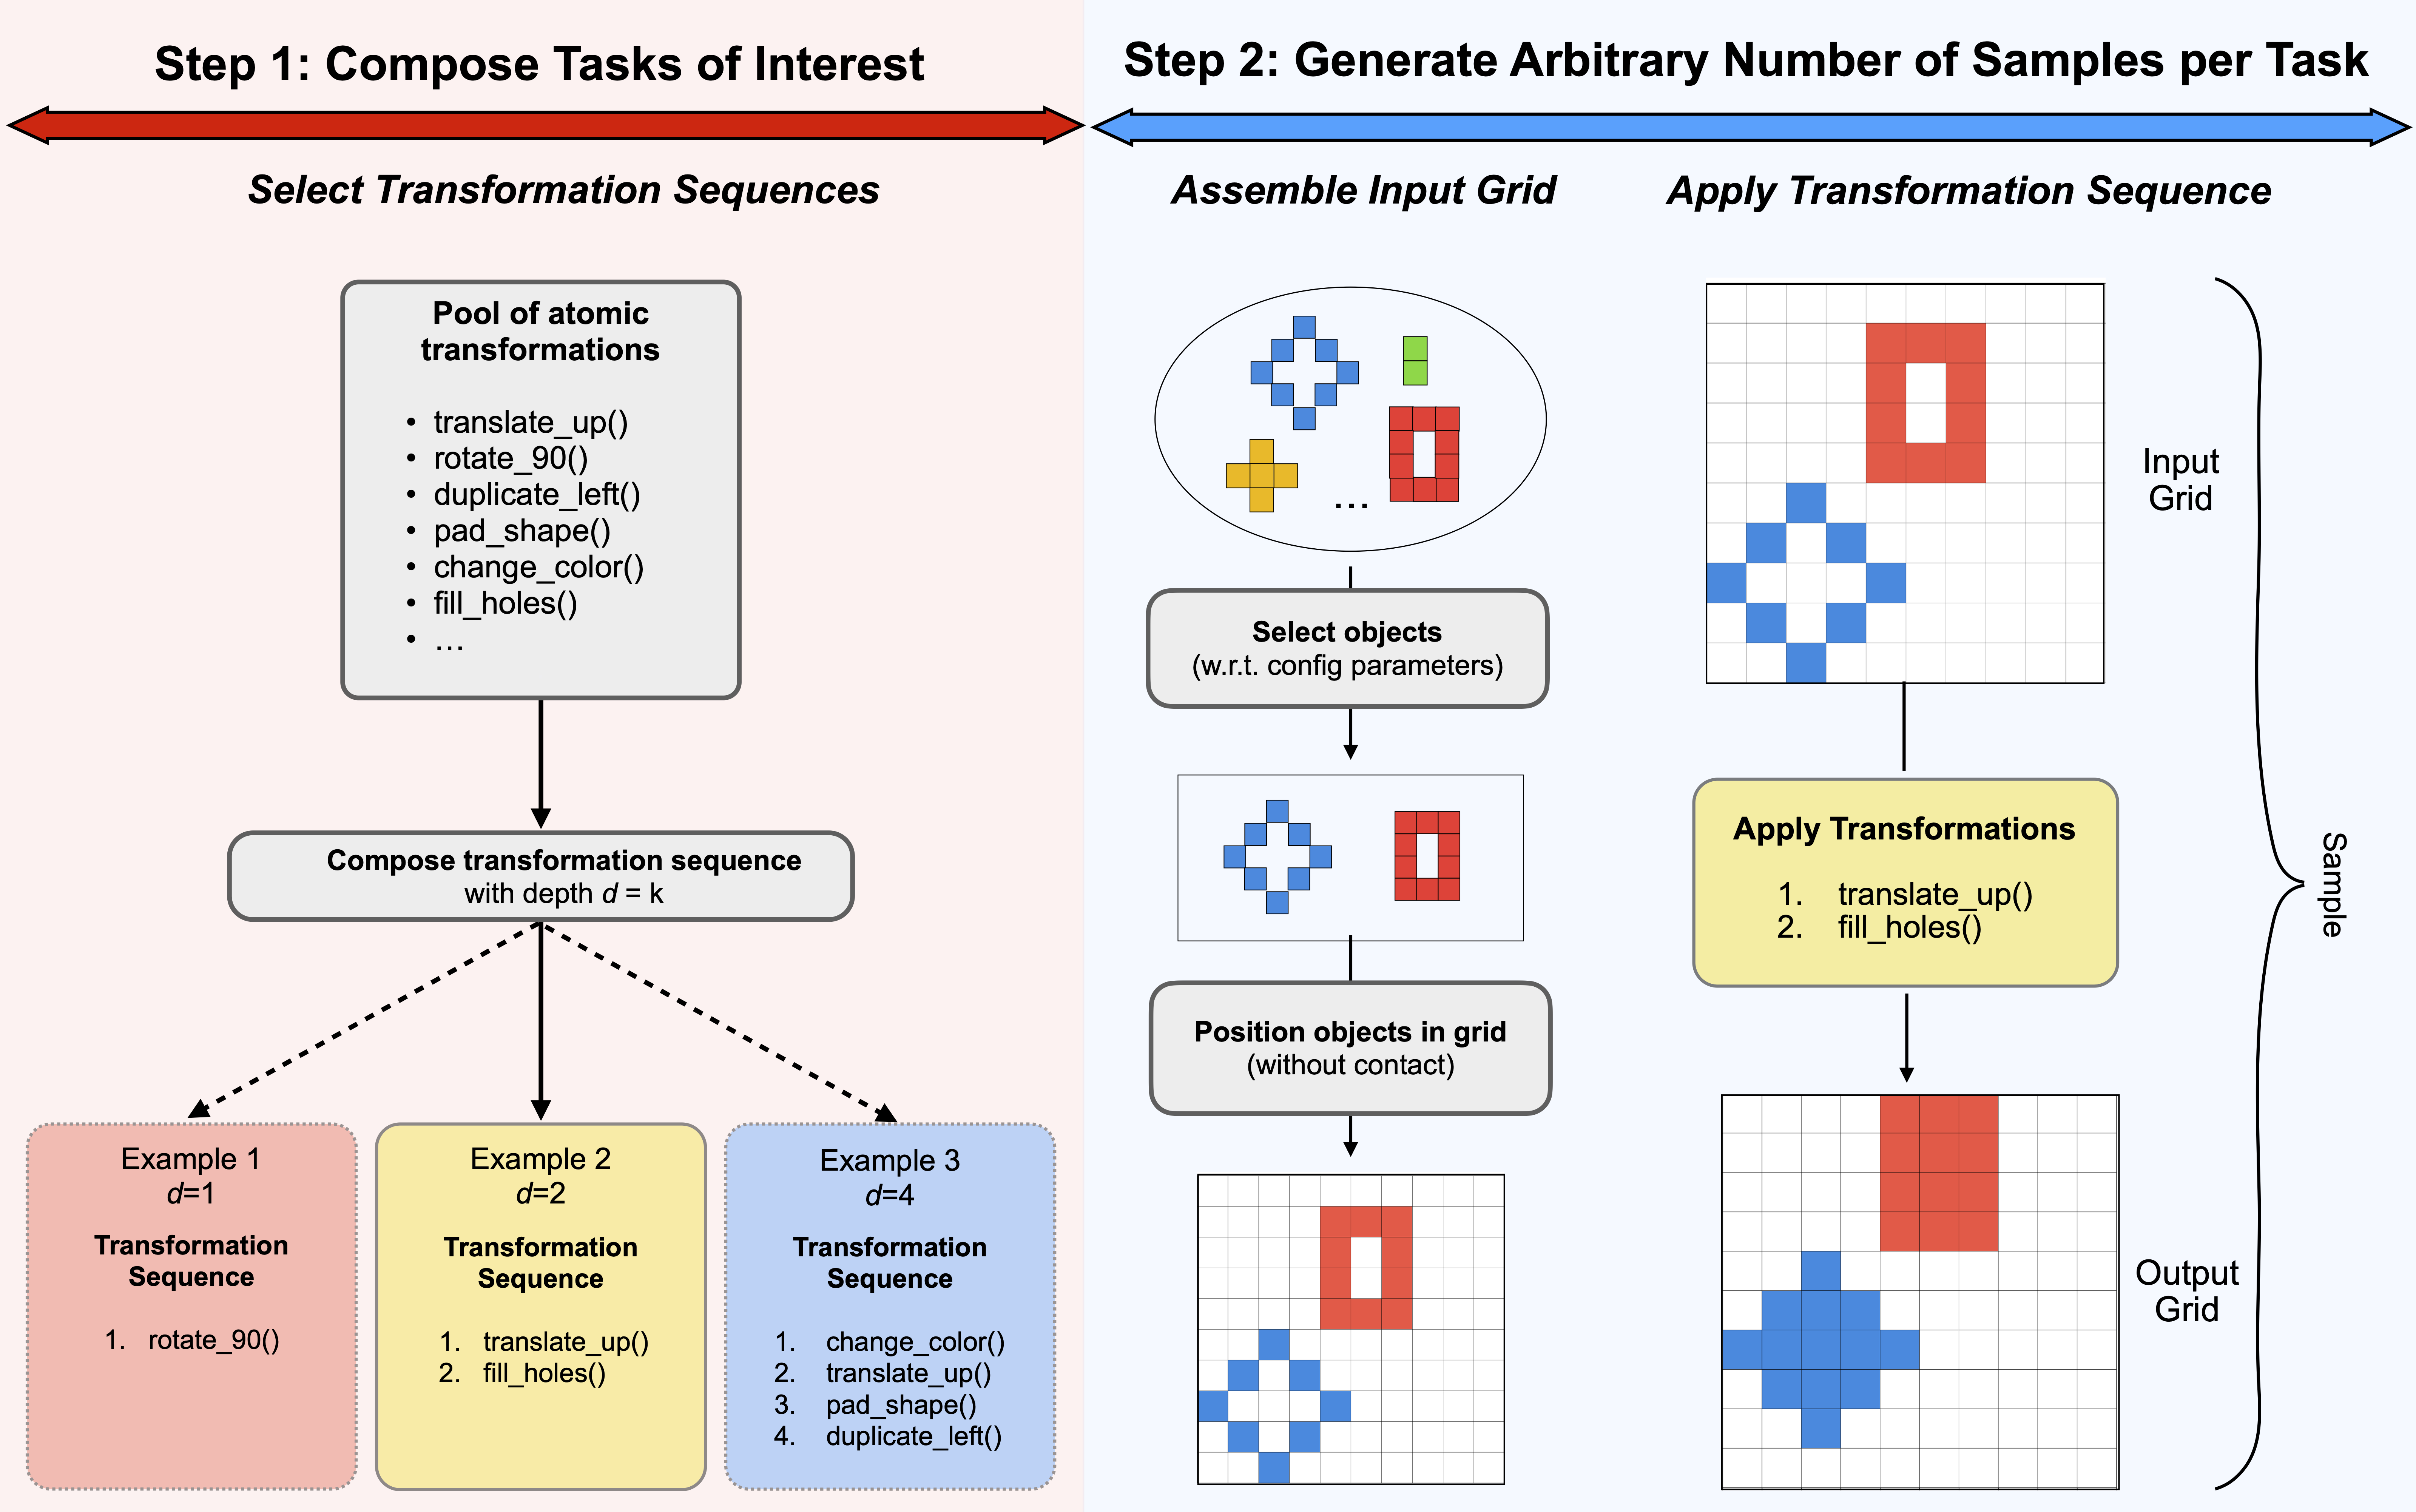
\includegraphics[width=1\columnwidth]{Figures/cogitao_figure.png}
    \caption{\generatorName\ is a Python-based procedural and object-centric data generator, inspired by the ARC-AGI \cite{cholletARC} grid-based environment. \generatorName\ samples transformation sequences, then, given the configuration requested by the user and the sampled transformations, randomly samples and position objects in an input grid. Once objects are positioned in the input grid, each transformation is sequentially applied to each object.}
    \label{fig:cogitao}
\end{figure}

\paragraph{COGITAO Generation} 

The generator can either randomly sample a sequence of transformations from a specified pool or use a user-defined sequence. After selecting the transformation sequence, it assembles random objects (w.r.t. config parameters) on the input grid, allowing each transformation to be applied to an output grid. 
Because some transformations (e.g., cropping) are irreversible and certain combinations are non-commutative, the order of transformations matters. With \ntransforms\ available transformations and a maximum transformation depth $k$, the theoretical upper bound on the number of distinct tasks is $N = n_{\text{transforms}}^{k} = \ntransforms^{k}$.
For example, at dept $d = 5$ and an adequate\footnote{``Adequate'' refers to grid and object configurations that avoid frequent generation failures—for instance, attempting to place ten objects in a $5 \times 5$ grid while performing four object transformations is impractical.} number of objects and grid size, the generator could theoretically create $n_{\text{tasks}} = \ntransforms^{5} \approx 1.7 \times 10^{8}$ unique tasks. 
Provided the grid is sufficiently large and generation time is not a limiting factor, the depth of compositional transformations can be arbitrarily large, making the space of possible tasks effectively unbounded. Further details on the generation method can be found in \ref{appendix:COGITAO_generation}.